%
% File eacl2017.tex
%
%% Based on the style files for ACL-2016
%% Based on the style files for ACL-2015, with some improvements
%%  taken from the NAACL-2016 style
%% Based on the style files for ACL-2014, which were, in turn,
%% Based on the style files for ACL-2013, which were, in turn,
%% Based on the style files for ACL-2012, which were, in turn,
%% based on the style files for ACL-2011, which were, in turn, 
%% based on the style files for ACL-2010, which were, in turn, 
%% based on the style files for ACL-IJCNLP-2009, which were, in turn,
%% based on the style files for EACL-2009 and IJCNLP-2008...

%% Based on the style files for EACL 2006 by 
%%e.agirre@ehu.es or Sergi.Balari@uab.es
%% and that of ACL 08 by Joakim Nivre and Noah Smith

\documentclass[11pt]{article}
\usepackage{eacl2017}
\usepackage{times}
\usepackage{url}
\usepackage{latexsym}
\usepackage{graphicx}

\eaclfinalcopy % Uncomment this line for the final submission
%\def\eaclpaperid{***} %  Enter the acl Paper ID here

%\setlength\titlebox{5cm}
% You can expand the titlebox if you need extra space
% to show all the authors. Please do not make the titlebox
% smaller than 5cm (the original size); we will check this
% in the camera-ready version and ask you to change it back.

\newcommand\BibTeX{B{\sc ib}\TeX}

\title{OpenNMT: Open-Source Toolkit for Neural Machine Translation}

\author{Yoon Kim$^*$, Guillaume Klein$^\dagger$, Yuntian Deng$^*$, Jean Senellart$^\dagger$, Alexander M. Rush$^*$ \\ Harvard University$^*$, Systran $^\dagger$d}

\date{}

\begin{document}
\maketitle
\begin{abstract}

  We describe an open-source toolkit for neural machine translation
  that supports research development of sequence-to-sequence models.
  The toolkit prioritizes simplicity, modularity, and efficiency to
  make it reasonable for researchers to experiment with variants of
  neural machine translation that explore different feature
  representations, model architectures, and source (multi)-modalities,
  while maintaining competitive performance and tractable training
  requirements. The toolkit consists of modeling and decoding support,
  as well as detailed pedagogical documentation about the underlying
  methodologies.

\end{abstract}

\section{Introduction}


Neural machine translation (NMT) is a new methodology for machine
translation \cite{}, that has shown remarkable gains particularly in
terms of human evaluation. Originally popularized by the work of
\cite{} and expanded upon by \cite{}. Over the last year the systems
have been further refined and developed by work such as \cite{}.

In this work we describe a new open-source toolkit for developing
neural machine translation systems, known as \textit{OpenNMT}. The
system is motivated by frameworks, such as Moses and CDec developed
for statistical machine translation (SMT). These toolkits aim to
provide a shared frameworks for developing and comparing open-source
SMT systems that are complete and flexible enough for research
development, while at the same time being efficient and accurate
enough to be used production contexts. 


Currently there are several existing NMT systems. Including Google NMT
\cite{}, ... Several of these systems are proprietary. Several others
are mainly research system such as seq2seq-attn. Perhaps most similar
to OpenNMT is the NeMaTus system \cite{}, based on the system of \cite{}
which aims to provide the same type of feature set as OpenNMT, using a
different underlying neural network toolkit.

In developing OpenNMT we prioritized three different factors, which
are described in this technical report: (1) Our top priority was
training and decoding speed. NMT systems are notoriously slow to
train, often requiring weeks of training time on the latest GPU
hardware and significant test resources. We targeted this issue by
implementing multi-GPU training, using aggressive memory sharing, and
developing a specialized CPU decoder. (2) Our second priority was system
modularity and teachibility. We intend OpenNMT as a living research
system, and so the codebase was developed to provide a
self-documenting overview of NMT. We discuss how this approach allowed
us to add factored models \cite{} to the system. (3) Finally NMT is a very 
quick moving research area, and we would like the system to support 
new research areas as they develop. To demonstrate this approach we 
abstracted out the core of OpenNMT as a library, and describe the case 
study of using OpenNMT for image-to-text translation. 

This report describes the background for NMT, the main aspects of system development, and the preliminary results from using the system in practice.  


\section{Background: Neural Machine Translation}

Neural machine translation has now been extensively described in many
excellent papers and tutorials \cite{}, which we briefly summarize. 
The arch


\begin{figure}
  \centering
  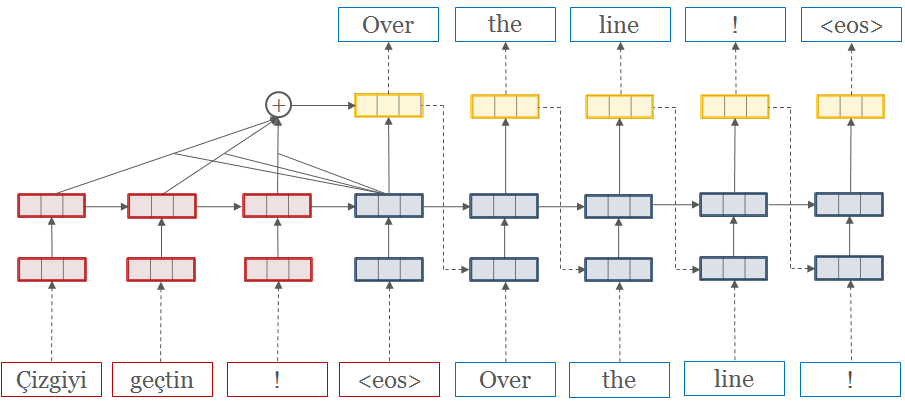
\includegraphics[width=\linewidth]{simple-attn}
  \caption{Schematic view of neural machine translation. The \textcolor{red}{red} source words are first mapped to word vectors and then fed into a recurrent neural network (RNN). Upon seeing the $\langle$eos$\rangle$ symbol, the final time step initializes a target \textcolor{blue}{blue} RNN. At each target time step, \textit{attention} is applied over the source RNN and combined with the current hidden state to produce a prediction $p(w_t| w_{1, \ldots, t-1}, x)$ of the next word. This prediction is then fed back into the target RNN.}
\end{figure}


\begin{itemize}
\item One column describing the technical details
\end{itemize}

\section{Implementation}

Details: torch. text-to-text mapping. toolkit for extensibility

\subsection{Modularity}

\begin{itemize}
\item Separate encoder/decoder 
\item Arbitrary input/output representations (features, images)
\end{itemize}

\subsection{Optimizations}

Encoder/Decoder optimization

\begin{itemize}
\item Shared memory (cite opt net)
\item C-Decoder  
\end{itemize}

\subsection{Advanced Features}

Other papers . 

\section{User Studies}

\paragraph{Feature-Based Inputs}

Discuss using modularity to add features as input and output

\paragraph{Knowledge Distillation/Pruning}

Discuss model access to allow for pruning and distillation. 

\paragraph{Im2Latex}

Discuss ability to modify encoder representation to allow for other tasks. 

\section{Experimental Results}

Mainly focus on NMT. Speed, memory, accuracy. 

\begin{table}
  \centering
  
  \caption{Performance Results. Several languages}
\end{table}


\begin{table}
  \centering
  
  \caption{Speed Results. Multi-GPU, distillation, c decoder}
\end{table}

Picture of demo application running 

\section{Conclusion}


\bibliography{writeup}
\bibliographystyle{eacl2017}


\end{document}
